\documentclass[journal]{IEEEtran}
% *** GRAPHICS RELATED PACKAGES ***
%
\ifCLASSINFOpdf
  % \usepackage[pdftex]{graphicx}
  % declare the path(s) where your graphic files are
  % \graphicspath{{../pdf/}{../jpeg/}}
  % and their extensions so you won't have to specify these with
  % every instance of \includegraphics
  % \DeclareGraphicsExtensions{.pdf,.jpeg,.png}
\else
  % or other class option (dvipsone, dvipdf, if not using dvips). graphicx
  % will default to the driver specified in the system graphics.cfg if no
  % driver is specified.
  % \usepackage[dvips]{graphicx}
  % declare the path(s) where your graphic files are
  % \graphicspath{{../eps/}}
  % and their extensions so you won't have to specify these with
  % every instance of \includegraphics
  % \DeclareGraphicsExtensions{.eps}
\fi
% graphicx was written by David Carlisle and Sebastian Rahtz. It is
% required if you want graphics, photos, etc. graphicx.sty is already
% installed on most LaTeX systems. The latest version and documentation can
% be obtained at: 
% http://www.ctan.org/tex-archive/macros/latex/required/graphics/
% Another good source of documentation is "Using Imported Graphics in


\usepackage[utf8]{inputenc}
\usepackage{amsmath}
\usepackage{amsfonts}
\usepackage{amssymb}
\usepackage{graphicx}
\usepackage{multicol}
\usepackage{algorithm}
\usepackage{algorithmic} 
\usepackage{subfig}
\usepackage{listings}
\usepackage[hidelinks]{hyperref} 
% correct bad hyphenation here
\hyphenation{op-tical net-works semi-conduc-tor}


\begin{document}
%
% paper title
% can use linebreaks \\ within to get better formatting as desired
\title{Retos que surgen con Big Data para el manejo y protección de información }

\author{Moreno~Vera,~Felipe*,\IEEEmembership{}
        Pecho~Chávez,~Augusto**,~\IEEEmembership{}
     	Tenorio~Trigoso,~Alonso***
\IEEEmembership{}
\thanks{*Felipe Moreno, Estudiante de Ciencia de la Computación UNI (felipe.moreno.vera@gmail.com). }
\thanks{**Augusto Pecho, Estudiante de Ciencia de la Computación UNI (augusto.pecho@uni.edu.pe). }
\thanks{***M.Sc. Alonso Tenorio, Profesor de Ciencia de la Computación UNI (atenoriot@uni.edu.pe). }
}


% The paper headers
\markboth{Big Data, Dic~2015}%
{Shell \MakeLowercase{\textit{et al.}}: Big Data}


% make the title area
\maketitle


\begin{abstract}
In this article we will provide some basics concepts about Big Data and Cyber Security in the current context, in addition we explain about the potential threats that appear next to the existence of Big Data.\\ \\
Next we explain about how the data is organized and protects and also the way we use Big Data for keep our systems secure and our information safe and the relation of this concept with Cyber Security.\\ \\
Finally we obtain a clear concept of how these two branches of research complement each other.\\

\end{abstract}


\begin{IEEEkeywords}
big data; cyber security; risks\\ \\
\end{IEEEkeywords}

\textbf{Resumen-En el presente artículo brindaremos algunos conceptos básicos sobre Big Data y Cyber Security en el contexto actual, además de las amenazas potenciales que aparecen junto a la existencia de Big Data.\\ \\
A continuación veremos cómo la data se organiza y se protege, además la forma en que utilizaremos Big Data para mantener nuestros sistemas seguros e información a salvo y la relación que tiene este concepto con Cyber Security dentro de una entidad (o empresa).\\ \\ 
Finalmente se obtendrá un concepto claro sobre cómo estas 2 ramas de investigación se completan entre sí.}\\ \\

\textbf{Palabras Clave: big data, cyber-seguridad, riesgos.}\\ 


\IEEEpeerreviewmaketitle



\section{Introducción}

\IEEEPARstart{U}{tilizar} Utilizar grandes cantidades de datos para gestionar las amenazas de seguridad debido a la magnitud de datos de la Internet y el hecho de que la población mundial está de manera constante en línea, se requieren proteger a los usuarios de la ciberdelincuencia que se pueden ver como un juego de números. Las mismas fuerzas que están impulsando Big Data están impulsando las amenazas al mismo tiempo. Nuevos métodos de cyber Board se necesitan  para procesar las amenazas  de la enorme cantidad de datos que surgen del mundo y mantenerse a la vanguardia de una sofisticada, agresiva y constante evolución panorámica de amenazas. Sin off-the-shelf solución puede abordar un problema de esta magnitud. La ampliación de gestionar los cambios es necesario ante el panorama de amenazas, pero se debe hacer de forma inteligente. Actualmente las compañías de seguridad de software necesitan no sólo detener los comportamientos maliciosos que ya se han iniciado, sino también predecir dicho comportamiento a futuro. Mejores Prácticas para lograr resultados finales (prototipos o interfaz GUI) para el usuario. Dirigiéndose al actual panorama de amenazas se requiere una relación sinérgica con los clientes y otras terceras partes que están expuestas constantemente a constante evolución de contenido malicioso. Una concesión de licencias, es un acuerdo que permite a los clientes a donar anónimamente datos sospechosos para su análisis y con la ingeniería inversa se puede proporcionar acceso valioso a los datos reales sobre máquinas reales que operan en el mundo real.\\ \\
Un ejemplo de Big Data y IA es que basándonos en datos recogidos de esta red comunitaria, los algoritmos de búsqueda especializados, aprendizaje automático, y el análisis pueden ser ejercidos sobre estos datos para identificar patrones anormales que pueden indicar una amenaza, pero eso son otros rubros.\\ \\
Herramientas de análisis de datos grandes serán la primera línea de defensa para proporcionar programas integrales e integrados de predicción de amenaza a la seguridad, detección y disuasión y prevención de acuerdo a recientes predicciones por el Instituto Internacional de Análisis (IIA) [7].\\ \\
FBR Capital Markets predice un aumento del 20\% en el "gasto de la seguridad cibernética de próxima generación" en el 2015, ya que las empresas se mueven más allá de los proveedores de cortafuegos y puntos finales tradicionales para la nube y soluciones de big data.\\ \\
Alrededor del 10\% de las empresas y agencias gubernamentales han actualizado a software de seguridad de última generación, tales como servidores de seguridad que detectan y bloquean las amenazas a nivel de aplicación, o grandes servicios de análisis de datos orientados a la seguridad, dijo el director gerente de FBR Capital Markets y Analista Senior de Investigación, Daniel Ives. "El mercado de esas herramientas de software podría ser de \$ 15 mil millones a \$ 20 mil millones durante los próximos tres años", añadió Ives.\\ \\
Los 5 peores riesgos de big Data, donde expone los 5 grandes riesgos que se presentan cuando la cantidad de datos en internet crecen y crecen sin un limite, las predicciones de los riesgos fueron realizadas por la organizacion EPIC [8].\\ \\
¿Quiénes son los vendedores que se aprovechan del análisis de grandes datos?
\subsection{IBM en análisis de seguridad cibernética}
IBM se llama a sí mismo el tercer jugador software de seguridad más grande en el mundo. Gartner lo ha calificado como el mayor proveedor de ventas de seguridad exclusivamente a empresas. IBM Security enfatiza la importancia de la analítica de cyber seguridad a sus clientes.\\ \\
"IBM está marcando el comienzo de una era de inteligencia impulsada por la seguridad de nuestros clientes", dice Brendan Hannigan, gerente general de IBM Security. "Con la tasa, el ritmo y la sofisticación de los ataques cibernéticos creciendo de manera exponencial, la seguridad se ha convertido en un problema de big data. El análisis en tiempo real es requerido como fundamento de la estrategia de seguridad de hoy en día. Socios de IBM con nuestros clientes a través de su C-Suite y Línea de Negocio desarrollan estrategias integradas e integrales de protección basada en análisis ", añade Hannigan.
\subsection{Splunk para la seguridad y fraude}
Splunk fue uno de los primeros motores en el gran espacio de análisis de seguridad de datos - y, como consecuencia, reclama una impresionante lista de clientes que utilizan su software para la seguridad y el fraude, incluyendo Adobe, Autodesk, Domino Pizza, First Data, Nordstrom, SAIC, Yahoo!, y muchos otros.\\ \\
Hay más de 200 aplicaciones de seguridad y complementos desarrollados por Splunk, sus socios o miembros de la comunidad para proporcionar información rápida en muchas de las tecnologías de seguridad líderes de la industria.\\ \\
Las líneas entre el análisis de seguridad y otros sectores de la seguridad están empezando a diferenciarse. Los vendedores con soluciones en torno a la red y el punto final de seguridad, inteligencia de amenazas, malware, identidad y autenticación, y otros, están alimentando datos en las plataformas de análisis. Blue Coat, Cisco, FireEye, Palo Alto Networks, Symantec, Tanium, y otros ofrecen ahora Splunk Apps.
\subsection{Actividad Inversora}
Los CVs [6] están en el juego de análisis de grandes datos, y aquí está parte de su reciente flujo de operaciones:\\
Sqrrl, un proveedor de análisis de datos grandes para identificar y responder a las amenazas cibernéticas, recaudó \$ 7 millones en la Serie B, dirigido por el Rally Ventures, junto con Atlas Venture y Matrix Partners. La compañía también dio a conocer un nuevo software destinado a detectar y responder a las amenazas de ciberseguridad. La financiación total hasta la fecha es ahora \$ 14.200.000.\\ \\
Endgame, un desarrollador de inteligencia y análisis de seguridad herramientas, recaudó \$ 30 millones en una tercera ronda. La ronda fue co-liderada por nuevos inversores Edgemore Capital y Top Tier Capital Partners. Partidarios anteriores Bessemer Venture Partners, Paladin Capital Group, Columbia Capital y Kleiner Perkins Caufield \& Byers también participaron, además de Savano Capital Partners.\\ \\
DB Networks, un proveedor de seguridad cibernética que aprovecha el aprendizaje automático y el análisis del comportamiento, recaudó \$ 17 millones en nuevos fondos de capital riesgo. La ronda fue liderada por Grotech Ventures, y acompañado por Khosla Ventures y Citi Ventures.\\ \\
Rapid7, un proveedor de software de seguridad y los servicios de análisis, cerró \$ 30 millones en fondos de Bain Capital y Technology Crossover Ventures. Rapid7 ha elegido a Morgan Stanley y Barclays para ayudar con una oferta pública inicial, según Reuters.
\subsection{Nuevos Entrantes}
La expectativa de ver un incremento de “jugadores” netos en big data y proveedores de inteligencia de negocios como los análisis de seguridad cibernética en el mercado aumenta.\\ \\
Hortonworks, una plataforma de código abierto para el almacenamiento y análisis de datos grandes, recaudó \$ 100 millones en su salida a bolsa con una capitalización de mercado inicial de \$ 666 millones. Sqrrl y Hortonworks van conjuntamente al mercado para proporcionar una plataforma de segura de big data basada en las capacidades de sus tecnologías complementarias.\\ \\
El más notable recién llegado al mercado es SAS Institute. La compañía de \$ 3 billones líder en el mercado de software de Business Analytics anunció recientemente su plataforma SAS Cybersecurity.

\section{Big Data Hoy en dia el entorno impone las tres Vs de Big Data: volumen, variedad y velocidad.}
Cada uno de éstos está aumentando a una velocidad asombrosa y ha requerido un cambio en cómo los proveedores de seguridad gestionan amenazas.
\subsection{Volumen: Una amenaza creciente}
El panorama de las amenazas está evolucionando de varias maneras, incluyendo el crecimiento en el volumen de amenazas. En la década de 1990, el usuario de la computadora personal en promedio recibio uno o dos mensajes de spam al día. En agosto de 2010, se estimó la cantidad de spam que alrededor de 200 mil millones de mensajes de spam enviados por día. Aumentos similares son características de las transferencias de archivos y el accseo a una página Web. En enero de 2008, la industria vio más malware en un mes que se había visto en los 15 años anteriores juntos. Trend Micro estima que el panorama de las amenazas para los usuarios finales ha experimentado un incremento de seis a siete órdenes de magnitud por encima sólo de los últimos años. Los números son desalentadores, pero esto es sólo la punta del iceberg. El cambio de protocolo de Internet actualmente en curso (de IPv4 a IPv6) está proporcionando los cibercriminales una nueva zona de juegos para explotar. Aproximadamente cuatro mil millones de direcciones IP únicas están disponibles para su uso con IPv4. Esto es un gran número todavía manejable. Por el contrario, IPv6 está proporcionando un número casi infinito de direcciones IP. La creciente demanda de direcciones IP únicas para los dispositivos que van desde televisores inteligentes a los teléfonos desarrollo motivado de las nuevas normas de IPv6. El objetivo era generar suficientes IP direcciones para evitar la necesidad de revisar más adelante el problema. Aunque IPv6 fija un solo problema, creado al mismo tiempo una enorme oportunidad para los cibercriminales y presentó una completamente nuevo conjunto de desafíos para la industria.
\subsection{Variedad: Métodos innovadores maliciosos}
El atractivo de la ganancia financiera ha motivado a los ciberdelincuentes para implementar nuevos métodos innovadores y ser más cuidadoso con cada año que pasa. Hoy en día, los cibercriminales son sofisticados, evolucionando su oficio y herramientas en tiempo real. Por ejemplo, el malware creado hoy a menudo sufre procedimientos de control de calidad. Los cibercriminales a prueba en numerosas máquinas y sistemas operativos para asegurarse de que no pasa por la detección. Mientras tanto, las amenazas polimórficas del lado del servidor en coche rápido evolución y propagación y son indetectables con los métodos tradicionales. Un centenar de piezas de malware puede ser multiplicado en miles de diferentes maneras. Y el malware ya no está restringido a los ordenadores personales. El malware multiplataforma significa que los dispositivos móviles también están en riesgo. Para agosto de 2012, hubo ataques de malware móviles donde ya 160.000 corresponden al año. En 2011 sólo había unos pocos.
\subsection{Velocidad: La fluidez de Amenazas}
La necesidad de gestionar, mantener y procesar este gran volumen y variedad de datos de forma regular base presenta los proveedores de seguridad con un reto de velocidad sin precedentes. La fluidez de la Internet a través del tiempo se suma a la complejidad del problema. A diferencia de una dirección física, que no puede ser trasladado sin dejar evidencia significativa detrás, el cambio de direcciones IP en la Internet es trivial, rápido y difícil de rastrear. Una empresa individual o una puede moverse sin esfuerzo y rápidamente de un lugar a otro sin dejar rastro.\\ \\
La determinación de si un sitio web en particular o una página contiene contenido malicioso es fluida a través del tiempo así como. Los cibercriminales se transforman de manera rutinaria sitios legítimos en sitios corruptos casi al instante. En un ejemplo de muchas de estas transformaciones, a principios de 2012, los cibercriminales han instalado un iFrame de redirección en un sitio de noticias popular en los Países Bajos. Lo que había sido un sitio web legítimo que mañana infectado a miles de personas a medida que examinaba el sitio comprometida durante su almuerzo horas.

\section{Metadata}
En el mundo se ha estado impulsando una iniciativa de datos abiertos para mover a los gobiernos a ser un administrador de datos. El objetivo en la liberación de los datos es la de servir mejor al público y promover el crecimiento económico a través de la reutilización de este datos. La dificultad en el uso de estos datos se deriva de la falta de las descripciones de metadatos. Reutilización de datos requiere la mayor cantidad de información posible sobre la procedencia de los datos; la historia completa de los métodos utilizados para la recolección, conservación, y el análisis. Los Metadatos adecuados aumentan las posibilidades de que los conjuntos de datos sean reutilizados correctamente, llevando a conclusiones analíticas que son menos propensos a ser defectuoso. Dos mecanismos se utilizan para la integración de datos en un modelo relacional. En el modelo relacional, tablas de búsqueda se establecen para traducir a un vocabulario común para las vistas, y una correspondencia uno-a-uno se utiliza para crear claves entre las tablas.\\ \\
En un entorno de NoSQL, se une no son posibles las búsquedas de modo de mesa y o claves no pueden ser utilizados para la integración de datos. La conexión de datos a través de bases de datos debe residir en la lógica de consulta y debe confiar en la información externa a los conjuntos de datos. Esta lógica de metadatos debe ser utilizado para seleccionar los datos relevantes para la integración y posterior análisis, lo que implica la necesidad de que tanto la representación estándar y atributos adicionales para lograr la recuperación de datos automatizado. Un segundo enfoque se utiliza para acelerar el proceso de integración de datos para mashups manuales de diversos conjuntos de datos.\\ \\
A menudo envolturas XML se utilizan para encapsular los elementos de datos, con la nomenclatura para cada conjunto de datos proporcionado en la envoltura, basándose en la interpretación de usuario de los elementos de datos. Este enfoque permite una rápida integración de los datos a través de las envolturas (a diferencia de una larga integración de almacenamiento de datos), pero no es un enfoque que puede ser automatizado, ni puede ser utilizada para los conjuntos de datos de gran volumen que no pueden ser copiadas por su volumen. Incluso en un mashup, términos de envoltura (encapsulación) utilizados en los metadatos son ellos mismos objeto de interpretación, por lo que la reutilización de elementos de datos difícil. Sin metadatos referidos a la terminología estándar dominios a través aplicables bien entendidos, los diversos conjuntos de datos no se pueden integrar de forma automática. Además, los elementos integrantes deben aplicarse fuera del gran almacenamiento de datos, lo que implica que la lógica de integración debe residir en la capa de metadatos.

\section{Los 5 peores riesgos de privacidad en Big Data}
La recopilación y manipulación de grandes volúmenes de datos, como sus proponedores han estado diciendo desde hace varios años, puede dar lugar a beneficios del mundo real: Los anuncios se centraron en lo que realmente se quiere comprar; coches inteligentes que pueden llamar a una ambulancia si estás en un accidente; dispositivos portátiles o implantables que pueden monitorear su salud y notificar a su médico si algo va mal.\\ \\
Pero, también puede llevar a grandes problemas de privacidad. Por ahora salta a la vista que cuando las personas generan miles de puntos de datos todos los días - a dónde van, con quién se comunican, lo que leen y escriben, lo que compran, lo que comen, lo que ven, lo mucho que ejercen, cómo mucho duermen y más - son vulnerables a la exposición de una manera inimaginable hasta hace una generación.\\ \\
Pasando a enumerar los 5 riesgos en Big Data:

\subsection{Discriminación}
Según EPIC, en comentarios hacia the U.S. Office of Science and Technology:” el uso de análisis predictivo para el sector público y privado, ahora puede ser usado por el gobierno y compañías para hacer determinaciones sobre la capacidad de hacer transacciones, de conseguir trabajo, separaciones o ver movimientos en tus tarjetas de crédito, el uso de nuestras asociaciones en análisis predictivo para tomar decisiones hacen negativo el impacto que tenemos de manera individual inhibiendo nuestra libertad de asociación”.\\ \\
El análisis de Big Data proporciona la capacidad para tomar decisiones discriminatorias que se hace sin la necesidad de que sea obvia o explicita las evidencias. Entonces a nivel de discriminación se tiene que: El riesgo más significativo es que se utiliza para ocultar la discriminación basada en criterios ilícitos, y para justificar el impacto desigual de las decisiones sobre las poblaciones vulnerables.

\subsection{Infracción, difusión e invasión de privacidad}
Big data, expone tus datos ante todo el mundo y cualquiera q tenga acceso a esta data, es libre de publicarla a su manera. Incluyendo casos como la empresa minorista Target y Home Depot, también la cadena de restaurante como PF, los mercados online como Chang o eBay, agencias gubernamentales, universidades, corporaciones en línea como AOL y el hackeo a Sony que no solo puso películas inéditas en la web, sino que expuso la información de miles de empleados, también los fraudes de tarjetas de créditos y la identidad de robo que es la más común entre todos estos puntos. Y Big data se encarga de exponer todos estos datos de los cuales pueden surgir numeroso informes de análisis.

\subsection{Adiós anonimato:}
Con big data, ahora es posible conectar todos los datos de una sola persona y cada vez que haya registro de alguna actividad de ella, puede ser conocida por cualquiera que tenga acceso a dicha data. Tus movimientos, transacciones, datos, podrían ser utilizados con fines maliciosos.\\ \\
Así como el facebook, twiter y otras redes más muestran y crean un perfil tuyo de preferencias, basta que des un “like” en un lugar equivocado o no apropiado, para que puedas ser filtrado a distintos tipos de categoría, dependiendo de tus gusto y además si esas categorías “no son las correctas socialmente” puede que tengas represalias hacia tu persona, e incluso si es que es una cuenta falta o una identidad doble.


\subsection{Exenciones de Gobierno}
Según EPIC, "los estadounidenses están en varias bases de datos del gobierno que nunca", incluida la del FBI, que recopila información de identificación personal (PII), incluyendo nombre, alias, raza, sexo, fecha y lugar de nacimiento, número de Seguro Social, pasaporte y el número de licencia de conducir, dirección, números de teléfono, fotografías, huellas dactilares, información financiera como cuentas bancarias, el empleo y el negocio de la información y más. Sin embargo, "aunque parezca increíble, la agencia ha eximido a sí mismo de la Ley de Privacidad (de 1974) los requisitos que el FBI mantienen sólo, registros personales de los precisos, pertinentes, oportunos y completos", "junto con otras garantías de que la información requerida por la Ley de Privacidad, dijo EPIC.\\ \\
En Big Data, al conocer los datos de todo sobre todo, puede que cuando haya alguna clase de selección o filtración, a la hora de concursar, o al momento de pedir algún trabajo o cualquier cargo importante en el gobierno, comúnmente a esto se le llama “tener contactos” los cuales dan referencias sobre tu persona, condición social, edad, dirección domicilio, etc etc...

\subsection{Falsificación de data o rompimiento de seguridad de datos:}
En big data al haber tantas proporciones de datos, se puede expresar estos peligros a nivel de negocios:
Numerosas empresas recogen y venden, "perfiles de los consumidores que no están claramente protegidos por los marcos legales vigentes", dijo EPIC.\\ \\
También hay poca o ninguna rendición de cuentas o incluso garantiza que la información sea exacta.\\ \\
"Los archivos de datos utilizados para el análisis de grandes datos a menudo pueden contener datos inexactos sobre las personas, los modelos de uso de datos que son incorrectos, ya que se refieren a individuos particulares, o simplemente ser defectuoso algoritmos".\\ \\
Aquí se ofrece varias otras medidas individuales para reducir sus riesgos de privacidad:\\ \\
*Dejar de compartir tanto en los medios sociales. "Si sólo tienes unas pocas personas que quieres ver fotos o vídeos, a continuación, enviar directamente a ellos en vez de publicar donde muchos pueden acceder a ellos", dijo.\\ \\
*No proporcione información a las empresas u otras organizaciones que no sean necesarios para los fines para los que usted está haciendo negocios con ellos. A menos que realmente necesitan su dirección y número de teléfono, no darle a ellos.\\ \\
*Utilice un navegador anónimo, como Hotspot Shield o Tor (The Onion Router) cuando visite sitios que podrían producir información que podría hacer que las personas sacan conclusiones inexactas acerca de usted.\\ \\
*Pida a los demás a no compartir información en línea acerca de usted sin su conocimiento. "Se puede sentir incómoda, pero hay que hacerlo", dijo.

\section{¿Dé donde vienen las amenazas?}
El perfil de amenaza cibernética es multifacético. Incluye malware, phishing, hacking, spam, ingeniería social, espionaje cibernético, móviles y amenazas internas, y eso no incluye los errores humanos tales como las fugas de datos accidentales o mal uso. Algunas de estas amenazas, como la piratería y el malware, han existido siempre junto a Internet; otras, específicamente las amenazas de usuarios generales, se han extendido debido a que las personas comunes han adoptado nuevas tecnologías más rápido de lo que los profesionales de TI han sido capaces de asegurarlos.\\ \\
Una encuesta, Figura 3, realizada a profesionales de TI muestran que el malware es la amenaza más abundante identificada en un 59\% de los casos, seguido del pishing (57\%), fuga de datos accidentales (44\%), hacking (43\%), spam (42\%), mal uso (40\%), violación de datos (40\%), ingeniería social (33\%), amenazas internas (25\%), cyber espionaje (25\%), amenazas móviles (23\%), errores (18\%) y amenazas físicas (17\%).

\begin{figure}[htb]
\centering
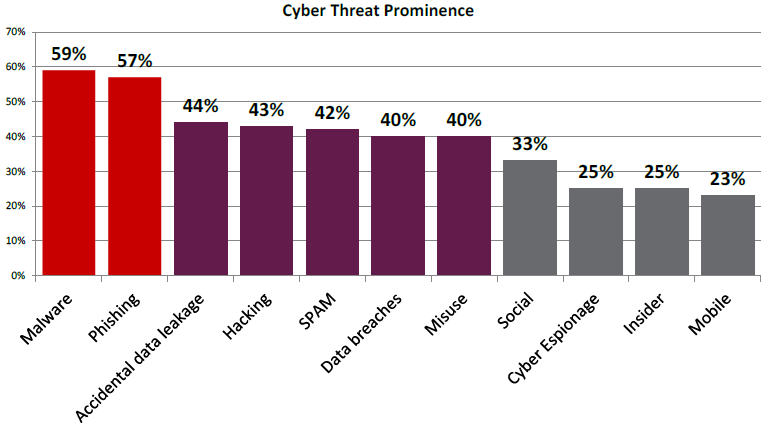
\includegraphics[width=0.40\paperwidth]{img1.png}
\caption{Proporción de cyber ataques}%\label{fig:horizonte}
\end{figure}

Las amenazas externas más comunes-malware, pishing, hacking, spam-son aquellas para las que los participantes de la encuesta se sienten mejor preparados. La buena preparación y alguna preparación ante estas amenazas alcanzan juntas el 95\% o más, y el porcentaje que se considera bien preparado es mayor que la proporción que se considera algo preparado.\\ \\
Significativamente, los profesionales del Departamento de Defensa y agencia de inteligencia de TI tienen el más alto grado de confianza para varios tipos de amenazas. Por ejemplo, el 83 por ciento de estos participantes en el estudio dijeron que estaban bien preparados y el 17 por ciento restante dijeron que estaban algo preparado para las amenazas de malware (Figura 4).

\begin{figure}[htb]
\centering
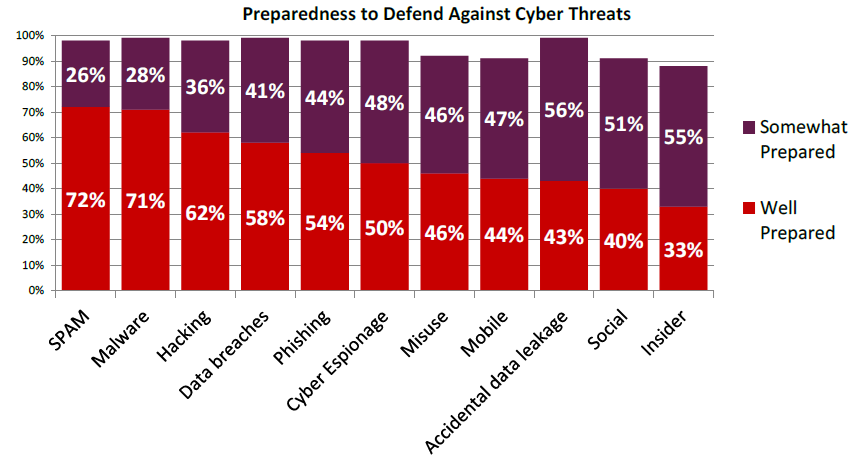
\includegraphics[width=0.4\textwidth]{img2.png}
\caption{Preparación para defenderse ante cyber ataques}%\label{fig:horizonte}
\end{figure}

Las amenazas de ingeniería social- engañando a un usuario de computadora a tomar algún tipo de decisión o divulgar información- son más difíciles de combatir. Todos los participantes del estudio, independientemente de la agencia de la cual provengan, son más propensos a ser algo preparados (51\%) en lugar de bien preparados (40\%). Las amenazas internas (55\%) y la fuga de datos accidentales (56\%) tienen a caer en su mayoría en el rango de algo preparados en vez de bien preparados (33\% y 43\%, respectivamente).\\ \\
Las amenazas móviles son el vector emergente. Sólo el 44\% de todos los participantes en el estudio creen que están bien preparados, mientras que el 47\% dice que son algo preparados. Esta es la categoría de amenaza con el porcentaje más bajo de preparación combinada, y refleja la rapidez con que la informática móvil está superando los mecanismos de seguridad establecidos, técnicas y educación.

\section{Aplicaciones en Cyber Security}
Aplicaciones prácticas para enfrentar los cyber ataques estarán disponibles en el futuro cercano. Las siguientes preguntas pueden ser respondidas con correctas implementaciones de la tecnología que brinda Big Data que abarcan una variedad de conjuntos de datos: ¿Qué datos están disponibles en los ataques del malware X a nivel global? ¿Qué puertos fueron atacados? ¿Qué usuarios fueron afectados? ¿Qué máquinas resultaron comprometidas? ¿Qué se filtró? ¿Se perdió información confidencial? ¿Quién lo hizo? ¿Era información nacional o extranjera? Preguntas más difíciles en el futuro serían: ¿Cuál es la actividad a nivel mundial de este atacante que se infiltró en mi perímetro? ¿Cuáles son todos los lugares de ataques del malware-name? ¿Qué debo esperar de este atacante durante la próxima hora, semana, mes? (basado en la data histórica del atacante). ¿Qué acciones inseguras llevan a cabo mis usuarios (clasificadas por significancia del riesgo)? ¿Qué actividad sospechosa ocurrió hoy? ¿Dónde está el mayor riesgo en el sistema? Estas preguntas resultan útiles para tabular estadísticas respecto a las vulnerabilidades frente a los ataques y poder visualizar los resultados.\\ \\
Este último conjunto de preguntas sobre el “futuro” requiere más investigación y desarrollo en temas como el aprendizaje automático y el razonamiento, y va mucho más allá del alcance de este artículo. Por ejemplo, ¿puede la ontología ayudarnos a pensar sobre el riesgo basado en la topología de los dispositivos y controles? En teoría, esto es determinístico y las máquinas deberían ser capaces de hacerlo mejor que el ser humano. Se puede modelar la seguridad del perímetro de una red de grandes empresas y recopilar datos en tiempo real, motivos del riesgo en tiempo real basados en la topología de dispositivos y controles, y responder a las amenazas en un intento por evitar pérdidas. ¿Dado el conjunto adecuado de datos y la generación de un conjunto de hipótesis razonables, podemos utilizar Big Data para hacer la recopilación de pruebas para apoyar o refutar las hipótesis de riesgos de seguridad y amenazas, a tiempo para evitar la pérdida?

\subsection{Progress to Date}
Como primer paso en la preparación para crear instancias de una ontología, debemos ser conscientes de lo que cientos de organizaciones hacen en el proceso de gestión de la seguridad cibernética actual en una empresa global en red. La descripción del flujo de trabajo está más allá del alcance de este artículo. La conciencia del sistema reside en la mente de cientos de profesionales que se encargan de investigar amenazas y malware, dar mantenimiento a los dispositivos de seguridad como firewalls y las configuraciones y parches de miles de dispositivos de red, monitorear eventos y archivos de registro, crear entradas cuando se observa una anomalía, y realizar acciones correctivas como  Incident Response; Configuration Management; Vulnerability and Patch Management; Firewall, Intrusion Detection and Prevention; Deep Packet Inspection and Cyber Threat Assessment; Security Architecture and Design; etcetera.\\ \\
Se pueden obtener todos los conocimientos necesarios de evaluación, decisión, planificación y respuesta en esta ontología.\\ \\
La gestión de la seguridad cibernética tiene las características de una exitosa obtención de conocimientos y el esfuerzo de la ingeniería ontológica. La información se encuentra en formato digital, y los procesos de seguridad cibernética son repetitivos, lo que significa que las mismas indicaciones de un ataque están bien documentados y se observaron en las operaciones rutinarias de red comunes y las medidas correctivas se documentan y se utilizan habitualmente. Esto no quiere decir que los expertos en seguridad cibernética no son muy bien informados y expertos, sino todo lo contrario. Este conocimiento puede ser codificado y se reutiliza, en esta parte la máquina lo hace mejor; el hombre debe seguir haciendo las partes que lo hace mejor que las máquinas. Con esta premisa, se puede pasar de una situación actual a una donde la defensa de la red está optimizad y sea eficiente, reduciendo el costo de la defensa, y haciendo está muy difícil y costosa para el atacante.

\subsection{Cyber ontología para contrarrestar ataques}
Los niveles más altos se ilustran en las figuras 3 y 4 que vienen a continuación.

\begin{figure}[htb]
\centering
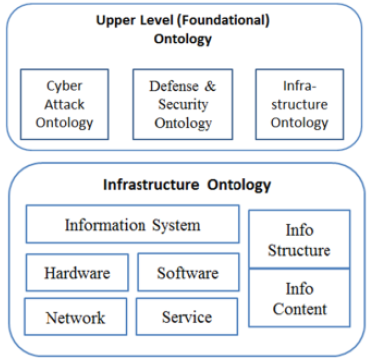
\includegraphics[width=0.4\textwidth]{img3.png}
\caption{Niveles superior e inferior en la infraestructura ontológica}%\label{fig:horizonte}
\end{figure}

\begin{figure}[htb]
\centering
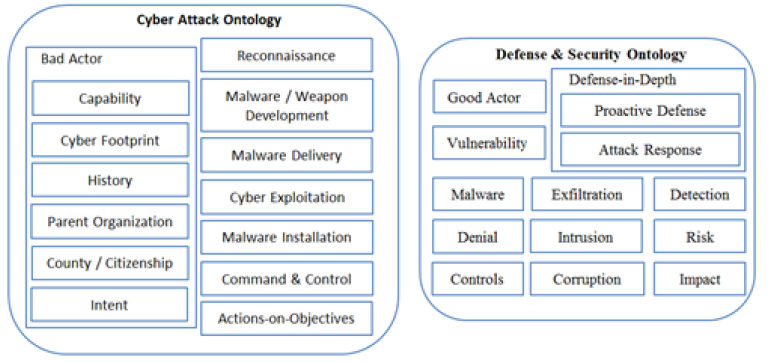
\includegraphics[width=0.4\textwidth]{img4.png}
\caption{Nivel inferior de ontología para ataque y defensa.}%\label{fig:horizonte}
\end{figure}

Un estudio sobre el comercio tendrá que ser llevado a cabo para poder disfrutar de herramientas que se pueden seleccionar para la implantación de un sistema de producción capaz de satisfacer los objetivos antes mencionados en una gran red empresarial global. Existen herramientas de ingeniería ontológica online como highfleet.com que proporciona una implementación de lógica de primer orden que es manejable (por restricciones de programación sencillas). Hay otras herramientas de ingeniería de la ontología, por ejemplo, el editor ontológico de descripción lógica Protégé.\\ \\
Debido a que esto está fuera del alcance de nuestro trabajo, no entraremos en detalles respecto a estas herramientas, pero algunos aspectos necesitan ser mencionados. Por ejemplo, hay muchos buenos recursos para especificar y ejemplificar estas ontologías a un nivel útil en la lucha virtual, los más notables son esfuerzos por MITRE [1]. Los temas de investigación siguen sin respuesta y se pueden clasificar en Big Data y Analyicsy, ontología y razonamiento probabilístico, toma de decisiones y diseño y arquitectura. La seguridad cibernética es un problema difícil de tratar, por otra parte, la sofisticación del ataque cibernético está avanzando rápidamente y agrava este problema de manera significativa.

\section{Ejemplos y aplicaciones}
El ejemplo de aplicación se basa en la data de hospitales brindado por el California HospitalMedical Center. Que contiene data sobre contaminantes del aire y personas que fueron afectadas siguiendo un tratamiento indicando su proporción de contaminantes en el cuerpo en un día cualquiera. Los contaminantes son sulfato y nitrato que se encuentran en el aire. 
Se presentan 2 análisis de data y filtrado de información.\\ \\
Funcion pollutantmean.R
Esta función retorna el promedio de contaminante de una persona alrededor de todos unos 3 años completos.\\
\lstset{language=Matlab, breaklines=true, basicstyle=\footnotesize}
\lstset{numbers=left, numberstyle=\tiny, stepnumber=1, numbersep=-2pt}
\begin{lstlisting}[frame=single]
  pollutantmean<-function(directory,pollutant,id=1:332){ 
  setwd(directory) 
   if((pollutant=="nitrate" || pollutant=="sulfate")&&(max(id)<=332)){ 
      x<-c() 
      id1<-as.character(id) 
      #### building files to read 
      for(i in 1:length(id1)){ 
         if(id[i]<10){ 
           id1[i]<-paste("00",id1[i],sep="") 
         } 
         if(10<=id[i] && id[i]<100){ 
           id1[i]<-paste("0",id1[i],sep="") 
         } 
      } 
      id1<-paste(id1,".csv",sep="") 
      data<-lapply(id1,read.csv)    
      #### calculating and retorning the mean  
      for(i in 1:length(data)){ 
         y<-data[[i]][pollutant] 
         y<-y[!is.na(y)] 
         x<-c(x,y) 
      } 
      Pollu.Mean<-mean(x) 
      return (Pollu.Mean) 
   } 
   else{ 
     print (" Pollutant or Id Error ") 
   } 
}
\end{lstlisting}

Función complete.R
Determina cuánta data está completa, eliminado o dejando de lado, aquellas que contengan datos null o vacíos.\\

\begin{lstlisting}[frame=single]
complete<-function(directory, id=1:332){ 
   setwd(directory) 
   if(max(id)<=332){ 
      x<-c() 
      id1<-as.character(id) 
#### building files to read 
      for(i in 1:length(id1)){ 
         if(id[i]<10){ 
           id1[i]<-paste("00",id1[i],sep="") 
         } 
         if(10<=id[i] && id[i]<100){ 
           id1[i]<-paste("0",id1[i],sep="") 
         } 
      } 
      id1<-paste(id1,".csv",sep="") 
      data<-lapply(id1,read.csv)    
      for(i in 1:length(data)){ 
         y<-data[[i]]["nitrate"] 
         y<-!is.na(y) 
         z<-data[[i]]["sulfate"] 
         z<-!is.na(z) 
         w<-y&z 
         w<-sum(w) 
         x<-c(x,w) 
      } 
      nobs<-x 
 
      table<-data.frame(id,nobs) 
      return (table) 
   } 
   else{ 
      print (" Id Error ") 
   } 
}
\end{lstlisting}
Se usó este ejemplo debido a que contiene una cantidad de data relevante a ser analizada y filtrada, dependiendo de las necesidades u operaciones a realizar con la data.

\section{Conclusiones}
Hemos visto que Big Data es una de las más grandes tendencias hoy por hoy, pero que trae consigo nuevas y cada vez más numerosas amenazas. También tenemos el conocimiento de cómo es que en otros países se hace negocio con Big Data y qué tan grande es la inversión para los fines de seguridad cibernética y análisis de datos.\\ \\
Se mostró una implementación sencilla pero bastante ilustrativa sobre el análisis y limpieza de data, lo cual es necesario para realizar una buena investigación de la historia de la data. También llegamos a la conclusión de que se requieren algoritmos 100\% eficientes, pues a medida que la data va incrementándose los tiempos de espera son cada vez más grandes, se requiere más memoria y no aceptan soluciones que tardan mucho tiempo en llegar.

\section*{Agradecimientos}
Agradecemos a la Escuela de Ciencia de la Computación de la Facultad de Ciencias (FC), de la Universidad Nacional de Ingeniería (UNI) por las facilidades brindadas para realizar nuestra investigación y al Centro de Tecnologías de Información y Comunicaciones (CTIC UNI) por el ambiente otorgado para la realización de la redacción y revisiones del presente artículo.


\ifCLASSOPTIONcaptionsoff
  \newpage
\fi

\begin{thebibliography}{1}

\bibitem{unistan} Obrst, L., Chase, P., Markeloff, R., Developing an Ontology of the Cyber-security Domain, Semantic Technology for Intelligence, Defense and Security (STIDS) 2012, GMU, Fairfax, VA, 2012\\
\bibitem{brid} Big data: The next frontier for innovation, competition, and productivity. James Manyika, Michael Chui, Brad Brown, Jacques Bughin, Richard Dobbs, Charles Roxburgh, and Angela Hung Byers. McKinsey Global Institute. May 2011.\\
\bibitem{par} Using Data for Systemic Financial Risk Management. Mark Flood, H V Jagadish, Albert Kyle, Frank Olken, and Louiqa Raschid. Proc. Fifth Biennial Conf. Innovative Data Systems Research, Jan. 2011.\\
\bibitem{parallel} LM Cyber Security and Transformational Technologies Keeping Systems and Data Safe.\\
\bibitem{paralelo2} Big Data Analytics for Security Intelligence 2013 Cloud Security Alliance – All Rights Reserved.\\
\bibitem{parallel3} CV: Capital de riesgo; \url{https://es.wikipedia.org/wiki/Capital_riesgo}\\
\bibitem{parallel4} Cybersecurity is the killer app for big data analytics by Steve Morgan \url{http://www.csoonline.com/article/2942083/big-data-security/cybersecurity-is-the-killer-app-for-big-data-analytics.html}\\
\bibitem{parallel5} The 5 worst Big data privacy risks; \url{http://www.csoonline.com/article/2855641/big-data-security/the-5-worst-big-data-privacy-risks-and-how-to-guard-against-them.html} \\

\end{thebibliography}


\end{document}



